\documentclass[12pt,letterpaper,fleqn]{article}
\usepackage{fullpage}
\usepackage[top=2cm, bottom=4.5cm, left=2.5cm, right=2.5cm]{geometry}
\usepackage{amsmath,amsthm,amsfonts,amssymb,amscd}
\usepackage[utf8]{inputenc}
\usepackage{lastpage}
\usepackage{enumerate}
\usepackage{fancyhdr}
\usepackage{mathrsfs}
\usepackage{xcolor}
\usepackage{graphicx}
\usepackage{listings}
\usepackage{hyperref}
\usepackage{amsmath}
\usepackage{nccmath}
\usepackage{physics}
\usepackage{float}

\newcommand{\R}{\mathbb{R}}
\newcommand{\Q}{\mathbb{Q}}

\newcommand{\cent}{$^{\circ}$}
\newcommand{\delfrac}[2][y]{\frac{\partial #1}{\partial #2}}


\hypersetup{%
 colorlinks=true,
  linkcolor=blue,
  linkbordercolor={0 0 1}
}
 
\renewcommand\lstlistingname{Algorithm}
\renewcommand\lstlistlistingname{Algorithms}
\def\lstlistingautorefname{Alg.}

\lstdefinestyle{Python}{
    language        = Python,
    frame           = lines, 
    basicstyle      = \footnotesize,
    keywordstyle    = \color{blue},
    stringstyle     = \color{green},
    commentstyle    = \color{red}\ttfamily
}

\setlength{\parindent}{0.3in}
\setlength{\parskip}{0.05in}

% Edit these as appropriate
\newcommand\course{Física - Frente 1}
\newcommand\hwnumber{1}                  % <-- homework number
\newcommand\NetIDa{netid19823}           % <-- NetID of person #1
\newcommand\NetIDb{netid12038}           % <-- NetID of person #2 (Comment this line out for problem sets)

\pagestyle{fancyplain}
\headheight 35pt
%\lhead{\NetIDa}
%\lhead{\NetIDa\\\NetIDb}                 % <-- Comment this line out for problem sets (make sure you are person #1)
\chead{\textbf{\Large Hidrodinâmica \hwnumber}}
\rhead{\course \\ Outubro/2020}
\lfoot{}
\cfoot{}
\rfoot{\small\thepage}
\headsep 1.5em

\begin{document}
\begin{enumerate}
    \item Uma pessoa, lendo o manual de uma ducha que acabou de adquirir para a sua casa, observa o gráfico, que relaciona a vazão na ducha com a pressão, medida em metros de coluna de água (mca).
    
    \begin{figure}[H]
        \centering
        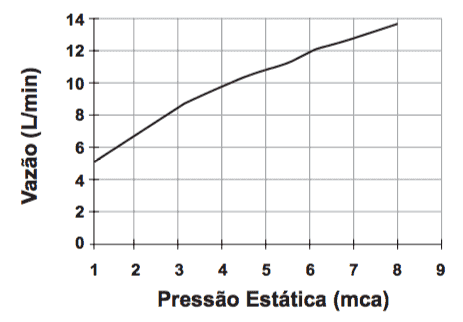
\includegraphics[width=0.6\textwidth]{ex_1.png}
    \end{figure}
    
    Nessa casa residem quatro pessoas. Cada uma delas toma um banho por dia, com duração média de 8 minutos, permanecendo o registro aberto com vazão máxima durante esse tempo. A ducha é instalada em um ponto seis metros abaixo do nível da lâmina de água, que se mantém constante dentro do reservatório. Ao final de 30 dias, esses banhos consumirão um volume de água, em litros, igual a
    \begin{enumerate}
        \item 69120
        \item 2880
        \item 8640
        \item 11520
        \item 17280
    \end{enumerate}
    
    \item Para oferecer acessibilidade aos portadores de dificuldade de locomoção, é utilizado, em ônibus e automóveis, o elevador hidráulico. Nesse dispositivo e usada uma bomba elétrica, para forçar um fluído a passar de uma tubulação estreita para outra mais larga, e dessa forma acionar um pistão que movimenta a plataforma. Considere um elevador hidráulico cuja área da cabeça do pistão seja cinco vezes maior do que a área da tubulação que sai da bomba.
    
    Desprezando o atrito e considerando uma aceleração gravitacional de $10m/s^2$, deseja-se elevar uma pessoa de 65kg em uma cadeira de rodas de 15kg sobre a plataforma de 20kg. Qual deve ser a força exercida pelo motor da bomba sobre o fluido, para que o cadeirante seja elevado com velocidade constante?
    
    \begin{enumerate}
        \item 20 N
        \item 100 N
        \item 200 N
        \item 500 N
        \item 1000 N
    \end{enumerate}
    
    \item Um bloco cúbico com 6 cm de aresta é parcialmente submersa em água até 1/3 de sua altura. Considerando-se que a aceleração da gravidade vale $10 m/s^2$ e sabendo-se que a massa específica da água vale $1000 kg/m^3$, calcule a intensidade do empuxo sobre o bloco, em Newtons.
    
    \item Observe, na figura a seguir, a representação de uma prensa hidráulica, na qual as forças $F_1$ e $F_2$ atuam, respectivamente, sobre os émbolos dos cilindros I e II.
    \begin{figure}[H]
        \centering
        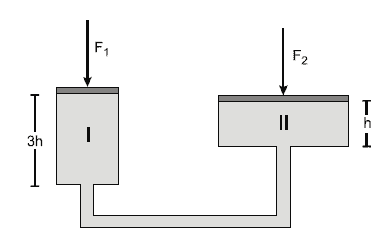
\includegraphics[width=0.6\textwidth]{ex_4.png}
    \end{figure}
    
    Admita que os cilindros estejam totalmente preenchidos por um líquido. O volume do cilindro II é igual a quatro vezes o volume do cilindro I, cuja altura é o triplo da altura do cilindro II. A razão $F_2/F_1$ entre as intensidades das forças, quando o sistema está em equilíbrio, corresponde a:
    \begin{enumerate}
        \item 12
        \item 6
        \item 3
        \item 2
        \item n.d.a
    \end{enumerate}
    
    \textit{Note e adote: Volume de um cilindro: $V = \pi r^2\,h$, em que '$r$' é o raio do cilindro e '$h$' é a altura}
    
    \item Em um recipiente contendo 100 mL (1,37 kg) de mercúrio líquido, são colocados dois cubos (A e B), com volumes de $2 cm^3$ cada, de um material inerte diante do mercúrio. Os cubos têm massas de 14 g e 20 g, respectivamente. Ao serem colocados no recipiente,
    \begin{enumerate}
        \item Ambos afundam até o fundo.
        \item O cubo A afunda, enquanto o B flutua.
        \item O cubo B afunda, enquanto o A flutua.
        \item Ambos cubos flutuam no meio do caminho até o fundo.
        \item Ambos cubos flutuam na superfície do líquido.
    \end{enumerate}
    
    \item Um reservatório contém um líquido de densidade $\rho_L=0,8 g/cm^3$. Flutuando em equilíbrio hidrostático nesse líquido, há um cilindro com área da base de $400 cm^2$ e altura de 12 cm. Observa-se que as bases desse cilindro estão paralelas à superficie do líquido e que somente 1/4 da altura desse cilindro encontra-se acima da superficie. Considerando $g = 10 m/s^2$, qual é o valor da densidade do material do cilindro?
    
    \item Um bloco de madeira impermeável, de massa M e dimensões $2 x 3 x 3 cm^3$, é inserido muito lentamente na água de um balde, até a condição de equilíbrio, com metade de seu volume submersa. A água que vaza do balde é coletada em um copo e tem massa m. A figura ilustra as situações inicial e final; em ambos os casos, o balde encontra-se cheio de água até sua capacidade máxima. A relação entre as massas '$m$' e '$M$' é tal que
    
    \begin{figure}[H]
        \centering
        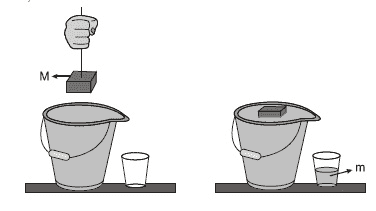
\includegraphics[width=0.6\textwidth]{ex_7.png}
    \end{figure}
    
    \begin{enumerate}
        \item $m=M/3$
        \item $m=M/2$
        \item $m=M$
        \item $m=2M$
        \item $m=3M$
    \end{enumerate}
    
    \item Um objeto homogêneo colocado em um recipiente com água tem 32\% de seu volume submerso; já em um recipiente com óleo, tem 40\% de seu volume submerso. A densidade desse óleo, em $g/cm^3$, é?
    
    \textit{Note e adote: densidade da água: $1g/cm^3$}
    \end{enumerate}
    
    \textbf{DESAFIO}: Um pedaço de gelo flutua em equilíbrio térmico com uma certa quantidade de água depositada em um balde. À medida que o gelo derrete, podemos afirmar que:
    \begin{enumerate}
        \item O nível da água no balde aumenta.
        \item O nível da água no balde diminui.
        \item O nível da água se mantém o mesmo
        \item Depende, pois o resultado pode mudar devido à temperatura do gelo/água, formato e massa do gelo
    \end{enumerate}
    Justifique a sua resposta.


\newpage
\section*{GABARITO}
\begin{enumerate}
    \item (d)
    \item (c)
    \item 0,72 N
    \item (a)
    \item (e)
    \item $d = 0,6\,g/cm^3$
    \item (c)
    \item $d=0,80\,g/cm^3$
    \item Traga o seu resultado para a monitoria para nós discutirmos.
\end{enumerate}
\end{document}
